\chapter{Fundamentos te\'oricos}
\label{cap:fundamentos}

En este capítulo se expone los conceptos importantes sobre el problema de predicción de la estructura tridimensional de la proteína (\textit{3-D PSP}) y su  estado del arte. 

\section{Problema de predicción de la estructura tridimensional de la proteína}

Este problema consiste en la predicción de las estructuras secundarias, terciarias y cuaternarias a partir de la estructura primaria (\citealp{Anfinsen:1973}).La estructura tridimensional de la proteína da importante información acerca de la función biológica de la proteína, ya que según su conformación estructural será su interacción con otras proteínas y moléculas. Es por ello que la solución a este problema se considera altamente importante para el área de desarrollo de fármacos y drogas, y para la biotecnología en el desarrollo de nuevas enzimas (\citealp{Cohen19961}).

\subsection{Estructura de la proteína}

Las proteínas son largas secuencias compuestas por 20 diferentes tipos de aminoácidos o residuos (ver tabla \ref{table:aminoacids}) unidos por enlaces peptídicos. Estos enlaces son la consecuencia de la unión de un grupo carboxilo de un aminoácido con el grupo amino de otro, produciéndose la liberación de una molécula de agua. Cada vez que se realiza un enlace peptídico la cadena comienza a crecer y a tomar forma debido a las fuerzas atómicas inherentes a este evento (\citealp{Anfinsen:1972}). En consecuencia, las estructuras comienzan a plegarse debido a las variaciones que se producen en los puntos de torsión de la proteína. Los ángulos en estos puntos se conocen como ángulos de torsión, y se les denomina con las letras griegas $\phi$ y $\psi$ a aquellos ángulos producidos por la unión de un átomo de Nitrógeno(\textit{N}) con un átomo de Carbono(\textit{C}), y un Carbono-alfa($C_{\alpha}$) con un Carbono(\textit{C}) respectivamente (\citealp{Anfinsen:1973}), tal como se puede apreciar en la figura \ref{fig:phi-psi-exam}.

\begin{table}[tp]
	\centering
	\caption[Listado de aminoácidos y sus códigos]{Listado de códigos de los 20 aminoácidos usados en el problema PSP}
	\begin{tabular}{|r|r|r|}
		\hline
		\textbf{Nombre residuo} & \textbf{Código 1 letra} & \textbf{Código 3 letras} \\ \hline
		Glicina 	        & G	& GLY	\\		
		Alanina 	        & A	& ALA	\\ 		
		Valina 	            & V	& VAL	\\  	
		Leucina 	        & L	& LEU	\\ 		
		Isoleucina 	        & I	& ILE	\\ 		
		Fenilalanina 		& F	& PHE	\\		
		Tirosina 			& Y	& TYR	\\	
		Triptófano 			& W	& TRP	\\
		Serina 	    		& S	& SER	\\	
		Treonina 			& T	& THR	\\	
		Cisteína 			& C	& CYS	\\
		Metionina 			& M	& MET	\\
		Ácido Aspártico     & D & ASP   \\
		Ácido Glutámico 	& E	& GLU	\\
		Histidina 			& H	& HIS	\\
		Lisina   			& K	& LYS	\\
		Arginina 			& R	& ARG	\\
		Asparginina 		& N	& ASN	\\
		Glutamina 			& Q	& GLN	\\
		Prolina 			& P	& PRO	\\ \hline
	\end{tabular}
	\label{table:aminoacids}
\end{table}

\begin{figure}[h]
	\centering
	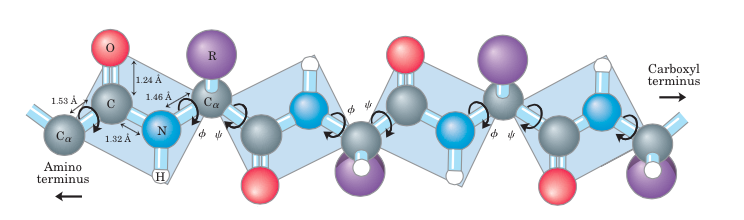
\includegraphics[scale=.6]{images/phipsi.png}
	\caption{\em \'Angulos de torsi\'on $\phi$ y $\psi$ (pág. 116 \citealp{lehninger}).}
	\label{fig:phi-psi-exam}
\end{figure}

Los cambios conformacionales de esta cadena son posibles debido a la rotación que ocurre en cada Carbono-\textalpha~($C_{\alpha}$). Además, cada aminoácido de la secuencia está polarizado, en otras palabras, tiene regiones positivas y negativas con un grupo \textit{C=O} libre, el cual puede actuar como receptor de un enlace de hidrógeno y un grupo \textit{NH} como donante de un enlace de hidrógeno.

Los 20 aminoácidos pueden ser clasificados de acuerdo a sus características químicas de la cadena lateral, que también juega un rol fundamental en la estructura 3-D. La Glicina, por ejemplo, tiene su cadena lateral más pequeña con solo un átomo de hidrógeno, lo que incrementa la flexibilidad de la estructura de la proteína (\citealp{Uzman:2001}). Por otro lado, la Cistina puede reaccionar con otra Cistina que se encuentre distante, de este modo, puede actuar como estabilizador de la estructura.

A raíz de lo anterior, estas cadenas se encuentras plegadas o enrolladas con una formación específica tridimensional, que pueden ser clasificadas en 4 niveles (\citealp{joao:1997}) y ser observadas en la figura \ref{fig:structures-protein}.

\begin{figure}
	\centering
	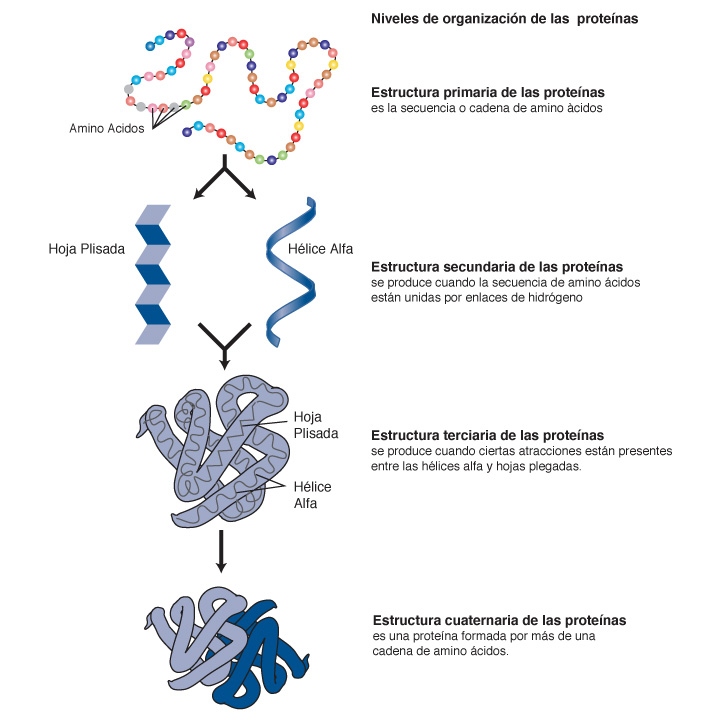
\includegraphics[scale=.6]{images/protein_lg.jpg}
	\caption{\em Niveles estructurales de la proteína (\citealp{image:genome-project})}
	\label{fig:structures-protein}
\end{figure}

\subsubsection{Estructuras Primarias y el Dogma de Anfinsen}
La estructura primaria de la proteína se define como el conjunto ordenado de aminoácidos dispuestos en forma de secuencia, a partir de la cual, tras la etapa de plegamiento (más detalle en la sección \ref{fundamentos:plegamiento}), se consolida la estructura a nivel funcional. Esto último se conoce como el \textit{Dogma de Anfinsen} (\citealp{Anfinsen:1973}) o \textit{Hipótesis de la termodinámica}. Por ejemplo, la proteína cuyo \textit{Protein Data Bank ID (PID)} es \textit{1K43} (\citealp{1k43}), tiene un largo de 14 aminoácidos, su estructura primaria viene dada por la representación lineal \textit{RGKWTYNGITYEGR}.

\subsubsection{Estructuras Secundarias y Clasificaci\'on STRIDE}
\label{cap:dssp}

Esta conformación molecular se forma por la presencia de patrones de enlaces de hidrógeno entre los átomos del grupo amino y carboxilo del polipéptido.

La organización estable de residuos de una proteína forman tipos de estructuras que son identificables. La formación de estas estructuras neutraliza los grupos polares en cada aminoácido. En el núcleo de la proteína las estructuras secundarias tienen un espacio limitado por lo que se encuentran cercas una de otra, debido a esto, el grupo lateral de cada aminoácido puede reaccionar con el de otro residuo. Esto es un factor a considerar en el modelado y alineamiento molecular (\citealp{molecular:book}).

Cuando se habla de estructuras secundarias de proteína, usualmente se usa la clasificación del código STRIDE que clasifica estas estructuras en 8 estados conformacionales (\citealp{stridepaper}).

%El código DSSP es el método estándar para asignar estructuras secundarias a los aminoácidos de la proteína y se basa en la detección de patrones de enlaces de hidrógeno, esta técnica fue inicialmente propuesta por \citealp{pauling:1951}. 

El funcionamiento de este algoritmo comienza por identificar los enlaces de hidrógeno implicados en la cadena principal (cadena de átomos enlazados con enlaces peptídicos) usando solamente su definición electrostática, asumiendo cargas parciales de \textit{-0.42e} y \textit{+0.20e} para el oxígeno del grupo carbonilo y el hidrógeno del grupo amida respectivamente. Los valores opuestos a estos son asignados al carbono del grupo carbonilo y al nitrógeno del grupo amida. Un enlace de hidrógeno es detectado si \textit{E} en la ecuación \ref{equation:ene-h} es menor que $-0.5kcal/mol$. 
\begin{equation}
	E=0.084*(\frac{1}{r_{ON}}+\frac{1}{r_{CH}}+\frac{1}{r_{OH}}+\frac{1}{r_{CN}})*332\frac{kcal}{mol}
	\label{equation:ene-h}
\end{equation}

Basado en esto, ocho tipos de estructuras secundarias pueden ser asignadas (ver tabla \ref{table:dssp}). La clasificación STRIDE establece un mínimo de residuos que participan en cada una de las estructuras secundarias. Por ejemplo, las conformaciones tipo hélices (G,H e I) y hojas requieren al menos 3.6 residuos adyacentes que deben formar parte del mismo patrón de enlaces de hidrógeno. Si la hélice u hoja es muy corta será designada como T o B respectivamente.

\begin{table}[h]
    \caption{Clasificaci\'on STRIDE y códigos asociados}
	\centering
	\begin{tabular}{|r|l|}
		\hline
		\textbf{Nombre estructura secundaria} & \textbf{Código STRIDE} \\ \hline
		$3_{10}$-helix 	& G		\\		
		$\alpha$-helix 	& H		\\ 		
		$\pi$-helix 	& I		\\  	
		$\beta$-bridge 	& B		\\ 		
		$\beta$-bulges 	& E		\\ 		
		Turn 			& T		\\		
		Bend 			& S		\\	
		Coil 			& C		\\		\hline
	\end{tabular}
	\label{table:dssp}
\end{table}


Para una simplificación de la definición, las 8 estructuras se pueden generalizar en cuatro:


\begin{itemize}
	\item \textbf{\textit{Hélices (Helix)}:} Las hélices ($3_{10}$-helix, $\alpha$-helix y $\pi$-helix ) corresponden al tipo más abundante de estructura secundaria. Las hélices tienen 3.6 aminoácidos por vuelta con un enlace de Hidrógeno formado cada 4 residuos; la longitud media es de 10 aminoácidos, no obstante, varía de 5 a 40 residuos por hélice (\citealp{molecular:book}). La alineación de los enlaces de H crea un momento dipolar de la hélice con una carga parcial positiva resultante en el extremo amino de esta. Debido a que esta región cuenta con grupos NH2 libres, puede interactuar con grupos cargados negativamente, tales como los fosfatos. La localización más frecuente de las hélices está en la superficie del núcleo de la proteína, proporcionando una interfaz con el entorno acuoso. La cara interna de la hélice tiende a tener aminoácidos hidrofóbicos, mientras que la cara externa tiende a ser hidrofílica. Por lo tanto, un tercio de 4 aminoácidos de la cadena tenderá a ser hidrofóbico, este patrón se puede detectar con bastante facilidad. Por ejemplo, las hélices a inmersas en el núcleo de la proteína o en las membranas celulares tienen una distribución más alta y regular de aminoácidos hidrofóbicos, por lo tanto, se pueden detectar y predecir con alta precisión. Las hélices expuestas en la superficie tienen una menor proporción de aminoácidos hidrofóbicos. Regiones con alta presencia de alanina, ácido glutamínico, leucina, metionina y baja de prolina, glicina, tirosina, serina tienden a formar una una hélice (\citealp{lehninger}).
	
	\begin{figure}[H]
		\centering
		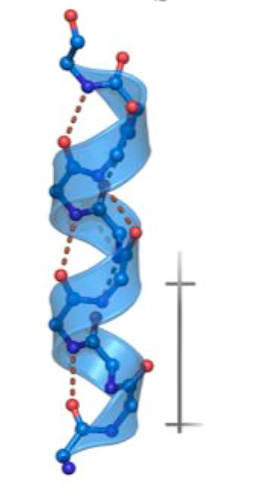
\includegraphics[scale=.4]{images/helix.png}
		\caption{\em Ejemplo de Hélice (pág. 25, \citealp{bioinfopt}).}
		\label{fig:helix}
	\end{figure}

	
	\item \textbf{\textit{Hojas (Sheets)}:} Las hojas se forman por enlaces de Hidrógeno entre un promedio de 5-10 aminoácidos consecutivos en una porción de la cadena con otra porción de 5-10 más abajo de la cadena. Las regiones que interactúan pueden ser adyacentes, con un lazo corto entre estas, o muy separados, con otras estructuras secundarias en  medio (\citealp{lehninger}). Cada hebra puede ir en la misma dirección para formar una hoja paralela, sin embargo, pueden tener dirección inversa para formar una hoja anti-paralela, o pueden estar mezcladas hojas paralelas con anti-paralelas para generar una hoja más compleja y mixta, ver figura \ref{fig:beta-sheets}. Cada aminoácido en las hebras interiores de la hoja forma dos enlaces de Hidrógeno con aminoácidos vecinos, mientras que cada aminoácido en las hebras externas forma solamente un enlace con la hebra interior (\citealp{molecular:book}).
	
	\begin{figure}[H]
		\centering
		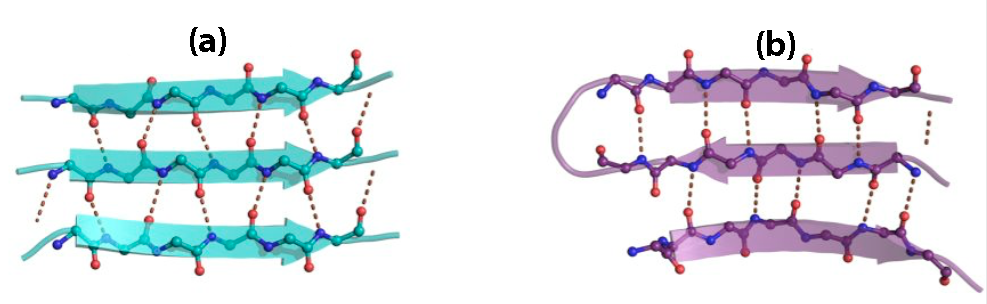
\includegraphics[scale=0.45]{images/beta.png}
		\caption{\em Ejemplo de \textbeta-hojas (a) paralela y (b) antiparalela (pág. 25, \citealp{bioinfopt}).}
		\label{fig:beta-sheets}
	\end{figure}

	\item \textbf{\textit{Vueltas (Turns)}:} Las vueltas son regiones de una cadena que se encuentran entre las hélices y hojas, de diferentes longitudes y configuraciones tridimensionales. Las vueltas en forma de U representan una vuelta completa en la cadena de polipéptido que une dos hebras (anti-paralelas o paralelas) y pueden ser tan cortas como dos aminoácidos de longitud (\citealp{molecular:book}).
	\begin{figure}[H]
		\centering
		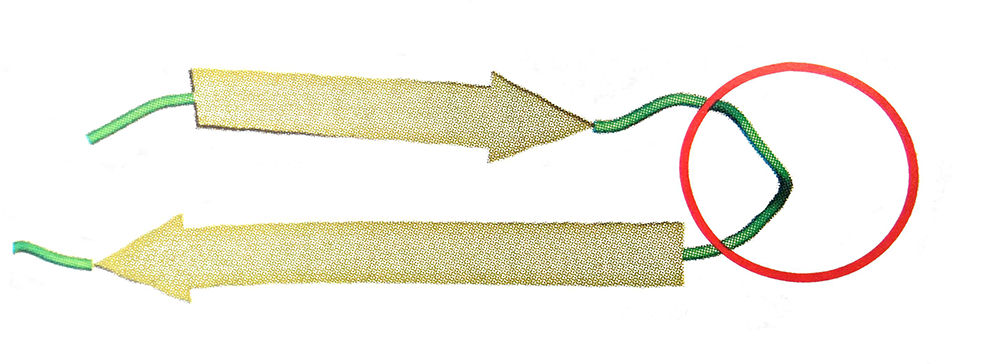
\includegraphics[scale=.8]{images/turn.png}
		\caption{\em Ejemplo de vuelta que se forma entre dos $\beta$-hojas (pág. 136, \citealp{book:kessel}).}
		\label{fig:turns}
	\end{figure}
	
	\item \textbf{\textit{Bobinas (Coils)}:} Las bobinas son aquellas secciones de la cadena de la proteína que no pueden ser clasificadas como hélices, hojas o vueltas (\citealp{molecular:book}).
\end{itemize}

%El código DSSP es una simplificación de la continuas variaciones de los patrones de enlaces de Hidrógeno presentes en una proteína. La mayoría de los métodos de predicción de estructuras secundarias simplifica aún más, llegando a una clasificación de 3 estructuras: hélices, hojas y bobinas. Los primeros métodos de predicción de estructuras secundarias estaban basados en cuán propenso era un aminoácido de formar parte de una hélice u hoja. Dichos métodos tenían una precisión del 60\% en la predicción de estos tres estados conformacionales (\citealp{Finkelstein:1971}). Al usar redes neuronales y máquinas vector de soporte, la precisión alcanzó valores mayores al 70\% (\citealp{Rost:1993}). Métodos posteriores logran hasta un 80$\sim$90\% de acierto (\citealp{Dor:2007}). La precisión de las predicciones de las estructuras secundarias juega un papel fundamental, ya que existen variados métodos que usan esta información como puntapié inicial para comenzar la predicción de las estructuras terciarias.

\subsubsection{Estructuras Terciarias}
\label{fundamentos:estructura-terciaria}

La estructura terciaria de la proteína tiene solo una cadena principal de aminoácidos y su principal característica es que se considera la posición espacial de cada átomo de la estructura (\citealp{branden:1999}). Puesto que se tiene esta información, se puede afirmar que la estructura terciaria corresponde al estado mínimo funcional de la proteína de la que se puede extraer conclusiones de sus propiedades biológicas, a través de su capacidad para interactuar con moléculas de otras proteínas o grupos celulares (\citealp{molecular:book}).

Esta estructura está compuesta por la unión de varias estructuras secundarias, que debido a interacciones que se mencionan posteriormente, se pliegan y distribuyen en el espacio dando forma al péptido. En la estructura terciaria, comúnmente los aminoácidos apolares se sitúan hacia el interior de la proteína, mientras que los polares hacia el exterior, lo que posibilita la interacción con los átomos de agua del medio acuoso. Por ejemplo, las proteínas integrales de membrana poseen a sus aminoácidos hidrofóbicos en la cara interna de la bicapa lipídica. Por lo tanto, la polaridad o apolaridad de los aminoácidos y su disposición influyen en las propiedades físico-químicas de la proteína (\citealp{branden:1999}).

\begin{figure}[H]
	\centering
	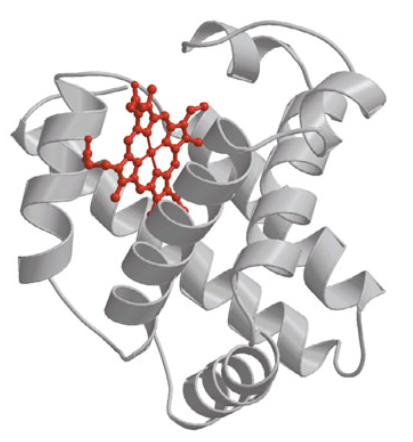
\includegraphics[scale=.5]{images/terciaria.png}
	\caption{\em Ejemplo de estructura terciaria: Mioglobina (pág. 133, \citealp{lehninger}).}
	\label{fig:ter-struct}
\end{figure}

Las interacciones que ocurren en la estructura terciaria de la proteína son cuatro (\citealp{branden:1999}):
\begin{itemize}
	\item Enlaces puentes de disulfuro entre Cistinas.
	\item Puentes de hidrógeno entre las cadenas laterales.
	\item Fuerzas e interacciones de \textit{van} der Waals.
	\item Efecto hidrofóbico de las móleculas.
\end{itemize}

Estas interacciones deben ser consideradas en la determinación y predicción de la estructura terciaria. Tal como se mencionó en la sección \ref{intro:enunciado}, este trabajo se concentra en la predicción de la proteína en su estructura terciaria. Los métodos experimentales más usados que dan información de la conformación de estos estados funcionales son los siguientes:

\begin{itemize}
	\item \textbf{Interferometría de doble polarización:} Este método se concentra en obtener información de la superficie de estas estructuras para determinar y monitorear los cambios conformacionales que sufre la proteína \cite[Cap.\ 11]{bioinfopt}.
	\item \textbf{Resonancia magnética nuclear:} Si bien, no provee una alta precisión como el método anterior, si puede indicar los cambios conformacionales que tiene una proteína en el medio \cite[Cap.\ 12]{bioinfopt}.
	\item \textbf{Cristalografía por rayos X:} Es la técnica más usada para determinar la estructura de la proteína. Provee información precisa del estado tridimensional pero no acerca de la flexibilidad conformacional \cite[Cap.\ 13]{bioinfopt}.
	
\end{itemize}

\subsubsection{Estructuras Cuaternarias}
Las estructuras cuaternarias son aquellas que poseen más de una cadena principal de polipéptidos, es decir, es la unión de dos o más estructuras terciarias (\citealp{branden:1999}), por lo que tienden a ser complejas estructuras funcionales.

Estas estructuras son de vital importancia biológica, ya que en base a ellas se realiza la construcción celular de, por ejemplo, microtúbulos, microfilamentos, capsómeros de virus y complejos enzimáticos que pueden activar o inhibir funciones biológicas (\cite[Cap.\ 4.3]{lehninger}). 

\subsection{Plegamiento de proteínas}
\label{fundamentos:plegamiento}

El plegamiento de proteínas (en inglés \textit{Protein folding}) es el proceso por el cual una proteína alcanza su estructura espacial. Como ya se ha mencionado, la estructura tridimensional marca las funcionalidades a nivel biológico (\citealp{Alberts:2002}), por lo que un incorrecto plegamiento implicaría una proteína inactiva o tóxica.

\begin{figure}[h]
	\centering
	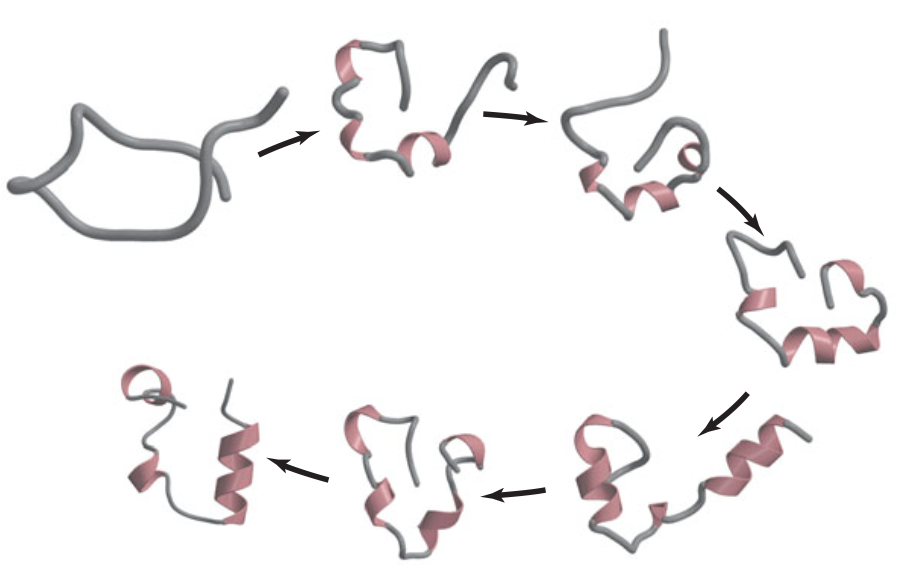
\includegraphics[scale=.5]{images/folding.png}
	\caption{\em Plegamiento de proteína (pág. 142, \citealp{lehninger}).}
	\label{fig:protein-folding}
\end{figure}

El proceso inverso al plegamiento se conoce como desnaturalización de proteínas. Una proteína que sufre este proceso deja de ser funcional al no tener una estructura tridimensional estable y definida. 

El plegamiento de la proteína se debe principalmente al medio en el que se encuentra y a los propiedades de los átomos y moléculas que la conforman. A medida que la proteína se pliega, pasa por etapas de plegamiento que asumen cambios en la energía global del sistema o estructura. Las variaciones energéticas se deben a factores termodinámicos como la entropía conformacional, los puentes de hidrógeno, las interacciones hidrofóbicas e hidrofílicas, y las interacciones de \textit{van} der Waals (\citealp{folding}). A continuación se definen brevemente estos conceptos.

\subsubsection{Entropía conformacional}

La conformación nativa de una proteína es la conformación de más baja energía libre de Gibbs. El proceso de plegamiento, como cualquier otro proceso biológico, se encuentra bajo control termodinámico y cinético, y es un proceso que está claramente favorecido en condiciones naturales. En otras palablas, el proceso de plegamiento hasta alcanzar la estructura nativa presenta un $\Delta$G negativo. Desde el punto de vista entrópico, el proceso de plegamiento supone una disminución neta de entropía desde la estructura denominada ovillo aleatorio (cuando la proteína está sin forma definida) a la única estructura nativa (estructura funcional). Este descenso de entropía, denominada entropía conformacional, supone un incremento positivo de energía libre en el proceso de plegamiento ($\Delta G = \Delta H – T\Delta S$). Para poder tener un descenso global en el proceso es necesario que el incremento de entalpía ($\Delta H$) sea negativo o que existan otros aumentos de entropía ($\Delta S$). La principal contribución entalpica al proceso de plegamiento la constituyen la formación de interacciones no covalentes que estabilizan la estructura nativa y las interacciones hidrofóbicas entre las cadenas laterales apolares que generalmente están localizadas al interior de la proteína (\citealp{entropia}).

\subsubsection{Enlaces de hidrógeno internos}

Un enlace de hidrógeno es la fuerza atractiva entre un átomo con carga negativa y un átomo de hidrógeno unido mediante un enlace covalente a otro átomo negativo, ver figura \ref{fig:h-bond}. 
\begin{figure}[h]
	\centering
	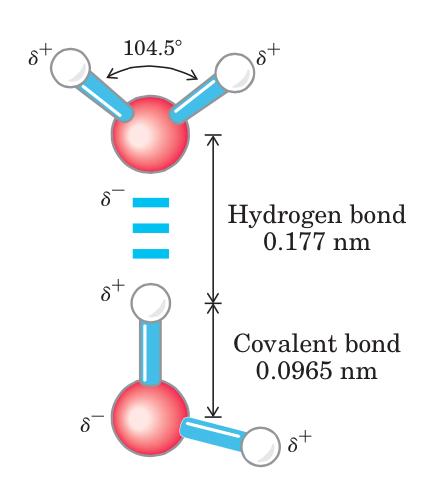
\includegraphics[scale=.5]{images/hidrobond.png}
	\caption{\em Enlace de hidrógeno (pág. 44, \citealp{lehninger}).}
	\label{fig:h-bond}
\end{figure}

Los patrones que forman estos enlaces  son lo usados por distintos métodos para poder predecir estructuras secundarias, actúan como estabilizadores lo que ayuda a la estructura terciaria a mantenerse definida (\citealp{hbond}).

\subsubsection{Fuerzas o Interacciones de \textit{van} der Waals}
Las fuerzas de \textit{van} der Waals son las fuerzas atractivas o repulsivas entre moléculas y/o átomos. Cuando se encuentran a una distancia moderada, las moléculas se atraen entre si, pero cuando sus nubes electrónicas empiezan a sobreponerse, las moléculas se repelen con fuerza (\citealp{entropia}). Ver gráfico figura \ref{fig:graph-vanderwaals}.
\begin{figure}[h]
	\centering
	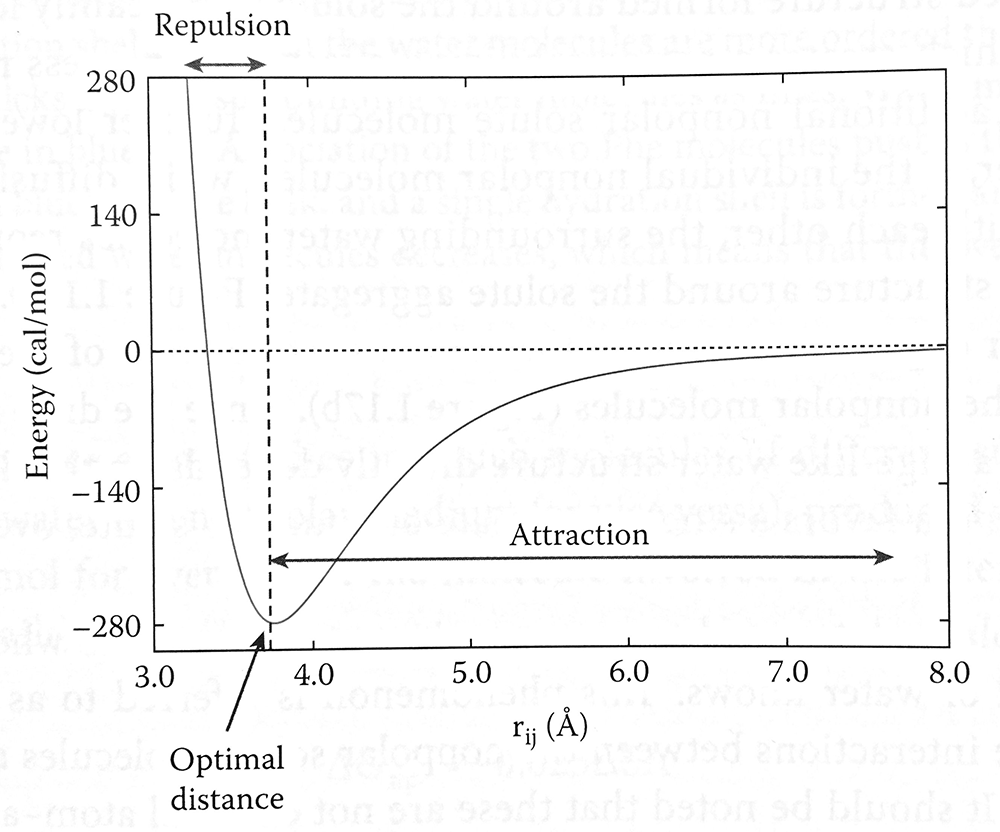
\includegraphics[scale=1]{images/vanderwaals.png}
	\caption{\em Gráfico de energía versus distancia entre átomos (pág. 55 \citealp{book:kessel}).}
	\label{fig:graph-vanderwaals}
\end{figure}

\subsubsection{Interacciones hidrofóbicas}

Toda sustancia hidrofóbica en contacto con moléculas de agua provoca fuerzas repulsivas produciéndose una separación entre estas. En el caso de las proteínas, los aminoácidos hidrofóbicos de las estructuras terciarias tienden a estar hacia el núcleo del polipéptido, lo que contribuye a un aumento de la entropía conformacional y a la estabilidad de la estructura al disminuir fuerzas repulsivas que generen cambios espaciales de los átomos  (\citealp{molecular:book}).

Luego de revisar los conceptos anteriores, se puede vislumbrar que minimizar el número de átomos o moléculas hidrofóbicas de la cadena lateral que están expuestas al agua, constituye una importante fuente de estabilización en el proceso de plegado. Además, la formación de enlaces de hidrógenos a nivel intramolecular de la proteína permite aumentar la estabilidad de la estructura, sin olvidar que la fuerza de estos enlaces de hidrógeno dependen del medio en el que se encuentran, de modo que, serán más fuertes si se encuentran en un medio hidrofóbico que en un medio hidrofílico (\citealp{molecular:book}).

\subsection{Campos de fuerza}

En el área de la Dinámica Molecular (\citealp{Karplus10052005}), un campo de fuerza se refiere al modelo de funciones matemáticas utilizadas para describir la energía potencial de un sistema de átomos y moléculas. Las funciones de campo de fuerza y el conjuntos de parámetros usados se derivan tanto del trabajo experimental y de cálculos de mecánica cuántica. Existen variados campos de fuerza propuestos por el mundo de la bioquímica y biofísica, pero para el presente trabajo se mencionará solo los campos \textit{Coarse grained}, que son los más utilizados en las predicciones de las proteínas, tienen la ventaja de representar mejor el medio y contexto en el que se desenvuelve la macro-molécula, por lo que proporcionan representaciones más fidedignas, esto aumenta la efectividad computacional (\citealp{hornak:2006}).

\subsubsection{Forma general de un campo de fuerza}

La forma de una campo de fuerza envuelve todos elementos unidos por enlaces (\textit{bonded terms}), que son aquellos átomos que están enlazados mediante enlaces covalentes, y los términos no enlazados (\textit{nonbonded terms}) que corresponden en su mayoría a fuerzas electrostáticas y de \textit{van} der Waals. Cada campo de fuerza tiene su propia fórmula matemática, pero se pueden generalizar de la siguiente forma.
\begin{equation}
	E_{total}=E_{bonded}+E_{nonbonded}
\end{equation}

donde:
\begin{equation}
E_{bonded}=E_{bond}+E_{angle}+E_{dihedral}
\end{equation}
\begin{equation}
\label{eq:nonbonded}
E_{nonbonded}=E_{electrostatic}+E_{van der waals}
\end{equation}

\subsubsection{Parametrizaciones de los campos de fuerza}

Cada campo de fuerza posee y se define con un conjunto de parámetros por cada tipo de átomo. Por ejemplo, un campo de fuerza podría tener distintos parámetros para un átomo de oxígeno en un grupo carbonilo y un grupo hidroxilo. Los parámetros más comunes incluyen la mása del átomo, el radio de \textit{van} der Waals y la carga parcial para los átomos, los valores correspondientes al largo de los enlaces, ángulos de estos y ángulos de torsión para pares, tripletas y cuadripletas de átomos enlazados. Los campos de fuerza más usados poseen cargas parciales fijas para los átomos debido que consideran que la electroestática del medio no interfiere en su carga. No obstante, se están desarrollando campos de fuerza que proponen la polarización de los átomos a causa de sus átomos vecinos (\citealp{Beauchamp:2012}).

\subsubsection{Deficiencias}

Todos los campos de fuerza se basan en aproximaciones numéricas derivadas de diferentes tipos de datos experimentales. Algunos de los campos de fuerza no contemplan la polarización del entorno, un efecto que puede reducir significativamente las interacciones electroestáticas sobre la carga parcial de los átomos (\citealp{hornak:2006}). Además, las fuerzas de \textit{van} der Waals están altamente ligadas al ambiente de la simulación, debido a las fuerzas que se originan de las interacciones de dipolos inducidos e instantáneos producidos entre el ambiente acuoso y las moléculas del péptido. 

Lo revisado anteriormente indica que la alta parametrización empírica provoca limitaciones de las simulaciones, produciendo sesgos y pérdida de precisión.

\subsection{Estado del Arte}
\label{fundamentos:estado-arte}

El foco de este trabajo está en el marco de predicción de estructuras terciarias de proteínas. En consecuencia, el estado del arte presentado da una visión general de las principales soluciones y técnicas usadas hoy en día para llevar a cabo dicho objetivo. Además, cabe mencionar los métodos actuales usados en la predicción de estructuras secundarias, ya que la solución propuesta en este trabajo hace uso de esa información.

Como dato adicional, cada dos años se realiza un experimento comunitario mundial llamado \text{\textit{CASP}} (\textit{Critical Assessment of Techniques for Protein Structure Prediction, Evaluación crítica de las técnicas para la predicción estructural proteica}) cuya función es dar a conocer métodos actuales de predicción y proveer una forma objetiva de evaluación de estos métodos (\citealp{casp:1995}). 

\subsubsection{Determinación de estructuras secundarias}

Uno de los primeros algoritmos propuestos en los años 70 fue el método de \textit{Chow-Fasman} \citealp{fasman:1974}, el cual se basa en la probabilidad de un residuo de pertenecer a cada tipo de estructura secundaria. Este algoritmo producía resultados con una precisión del 50$\sim$60\%, la baja precisión se debe a la cantidad de reducida de información disponible en esa época. Unos años más tarde, el método de GOR (\citealp{garnier:1978}) permitía obtener una precisión del 60 a 65\% al incorporar al algoritmo de Chow-Fasman la influencia de los residuos vecinos en la probabilidad de formar una cierta estructura secundaria. El siguiente avance significativo viene con el uso de redes neuronales (\textit{Neural Networks, NN}) y máquinas vector de soporte (\textit{Support Vector Machine, SVM}) aumentaron la precisión por sobre el 70\% (\citealp{Rost:1993}) llegando a alcanzar el 90\% (\citealp{Dor:2007}). En la actualidad gracias a internet, es posible acceder a herramientas tipo NN como \textit{PSIPRED SERVER} (\citealp{psipred:2013}) basado en el algortimo \textit{PSIBLAST} (propuesto en \citealp{psiblast:1997}) alcanzando una precisión de 81.6\%, y \textit{JPRED 3 SERVER} (\citealp{jpred:2008}) que hace uso del algoritmo \textit{JNET} (\citealp{jpred:2000}) con un 81.5\%. Para determinar las estructuras secundarias de las proteínas usadas en este trabajo, se hace uso de STRIDE (\citealp{stride:2004}) el cual fue revisado en la sección \ref{cap:dssp}.

\subsubsection{Predicción de estructuras terciarias}

La predicción de estructuras terciarias continua siendo un problema de extrema dificultad. Los dos principales problemas de la simulación es el cálculo de la energía libre de la proteína y función de minimización de energía. Los métodos de predicción deben explorar el espacio de soluciones para encontrar la estructura que cumple los requisitos planteados anteriormente, el problema recae en el espacio de búsqueda que resulta ser muy amplio a medida que la cadena de residuos aumenta, lo que hace intratable el problema debido al costo computacional que conlleva. Estos problemas pueden ser aminorados parcialmente usando técnicas de modelado por homología y enhebrado de secuencias, cuyo fundamento se basa en asumir que si se tiene la estructura generada de una secuencia, al tener la misma secuencia en otra proteína tenderá a formar una estructura similar (\citealp{Zhang:2008}).

Los enfoques actuales para predecir la estructura terciaria de la proteína según son cuatro (\citealp{Dorn2014251}), planteados a continuación.

\subsubsection{Métodos ab initio sin información de bases de datos}
Los métodos \textit{ab initio} o \textit{de novo} son técnicas de modelamiento que buscan construir la estructura tridimensional de la proteína simulando los procesos termodínamicos que ocurren a nivel biológico (\citealp{floudas:2006}). Intentan reproducir el comportamiento y las etapas de plegado de la proteína mediante la minimización de la energía libre del sistema haciendo uso de eventos moleculares. A medida que la cantidad de residuos aumenta, la cantidad de recursos computacionales necesarios en este método se incrementa debido a la complejidad del problema (\citealp{Crescenzi:1998}). Se han creado supercomputadoras específicamente para resolver este problema usando métodos \textit{ab initio}, como \textit{BLUE GENE} (\citealp{bluegene:2001}) y \textit{MDGRAPE-3} (\citealp{mdgrape:2003}) o amplias estructuras distribuidas, como el proyecto \textit{ROBETTA} (\citealp{robetta}).

\subsubsection{Métodos ab initio con información de bases de datos}
\label{fundamentos:abinitio-db}
Los métodos basados en \textit{ab initio} que utilizan información de base de datos son una variante del método anterior, ya que la principal diferencia radica en que usan información experimental para crear una estructura inicial más acabada, pudiendo ser refinada usando técnicas de Dinámica Molecular \citealp{floudas:2006}. Algunos de los métodos actuales son \textit{I-TASSER} (\citealp{itasser:2015}), \textit{ANGLOR} (\citealp{anglor:2008}) y \textit{FRAGFOLD} (\citealp{fragfold:2001}) y \textit{ROSETTA} (\citealp{rosseta:2010}).


\subsubsection{Métodos de enhebrado}
Estos métodos usan la alineación de secuencia con una base de datos para obtener estructuras conocidas que después irán uniendo a la predicción (\citealp{floudas:2006}). El principal problema de esta técnica es la búsqueda de secuencias en las bases de datos, ya que una secuencia de una estructura puede estar presente en las bases de datos experimentales más de una vez y con distintas conformaciones espaciales. Otro problema ligado a las técnicas de alineación es el largo de la secuencia a buscar, ya que al aumentar, las posibles combinaciones de sub-secuencias crece de manera considerable (\citealp{lathrop:1994}). Herramientas disponibles de esta área son \textit{GENTHREADER} \citealp{genthreader:1999}, \textit{PROSPECT} \citealp{kim:2003} y \textit{HHpred} (\citealp{soding:2005}).


\subsubsection{Métodos de modelado por comparación}
Los métodos de modelado por comparación se basan en el principio de que las estructuras secundarias se conservan más evolutivamente que las secuencias de aminoácidos que las generan (\citealp{floudas:2006}). Por  ejemplo, si se tiene una estructura secundaria tipo hélice con 10 residuos, el método buscará en las bases de datos hélices con una cantidad de residuos similar (sin importar cuales sean), y mediante una función de fitness escogerá la mejor estructura tridimensional para la predicción. Ejemplos de este método son \textit{MODELLER} (\citealp{eswar:2002}), \textit{CLUSTALW} (\citealp{clustalw}) y \textit{COMPASS} (\citealp{compass}).

\section{Algoritmos meméticos}

En el mundo de la informática, existen métodos de resolución de problemas de optimización que permiten encontrar soluciones cercanas al óptimo global (mínimo o máximo según corresponda), estos métodos son llamados metaheurísticas y son usados generalmente cuando el problema no puede ser resuelto con métodos tradicionales ya que las implementaciones pueden ser impracticables y demasiado costosas a nivel computacional. Dentro de este conjunto de técnicas se encuentran los algoritmos meméticos.

\label{fundamentos:memeticos}

\subsection{Definición}
Un algoritmo memético (\textit{Memetic Algorithm, MA}) es una metaheurística evolutiva basada en población que usa un operador de búsqueda local para el refinamiento de sus soluciones (\citealp{moscato:2011}). El nombre proviene de la palabra \textit{meme} la que puede entenderse como un objeto cultural que es transmitido por repetición y replicación de manera análoga a la transmisión biológica de genes (\citealp{meme:2015}).

\subsection{Estructura}

El algoritmo \ref{alg:memetico-gen} muestra la estructura general de un MA genérico. Los algoritmos meméticos están compuestos por operadores evolutivos más un operador de búsqueda local. Estos operadores actúan sobre agentes que componen la población, esta es la principal diferencia con los algoritmos evolutivos que hacen uso de individuos. La diferencia entre individuo y agente radica en que el primero es un ente pasivo que está sujeto a procesos y reglas evolutivas, mientras que un \textit{agente} es un ente activo que busca mejorar haciendo uso de la información propia del problema (a través de la búsqueda local) (\citealp{moscato:2011}).

En primer lugar, los algoritmos meméticos deben inicializarse con una población inicial de soluciones (lineas 2 al 5, algoritmo \ref{alg:memetico-gen}), que generalmente son obtenidas por funciones aleatorias, lo que deja de manera implícita que no se preocupan de la calidad ni eficiencia de la solución. Una vez que se tiene la base de la población sobre la cual se va a iterar, (cada iteración sobre la población se conoce como generación) se realiza el ciclo generacional para hacer evolucionar el sistema (lineas 7 al 25, algoritmo \ref{alg:memetico-gen}) o converger a soluciones prometedoras que sean iguales o cercanas al óptimo global del problema en cuestión (\citealp{hugo}). Las líneas 10 al 13 corresponden a la etapa de cruzamiento, en esta se escogen las soluciones a cruzar. Luego, la línea 14 muestra la acción del operador de búsqueda local, esta etapa es vital en los algoritmos meméticos por definición, ya que es en donde se aplica el conocimiento acerca del problema para conducir a mejores soluciones. Posteriormente, continua la etapa de mutación que brinda de diversidad a la población y permite escapar de mínimos locales (lineas 16 al 18, algoritmo \ref{alg:memetico-gen}). Los criterios de fin de las generaciones pueden ser variados, a modo de ejemplo, se puede elegir que termine cuando se alcanzan 100 generaciones o que el tiempo de ejecución sea de 10 horas.

\begin{algorithm}[ht]
	\begin{algorithmic}[1]
		\REQUIRE una instancia \textit{I} de un problema \textit{P}
		\ENSURE una solución \textit{sol}
		\STATE		\COMMENT Población inicial
		\FOR {$j \leftarrow 1:popsize$}
		\STATE $ind \leftarrow $GenerarSol(\textit{I})
		\STATE $pop[j] \leftarrow$ MejoraLocal(\textit{ind})
		\ENDFOR
		\STATE \COMMENT Ciclo Generacional
		\REPEAT
		\STATE \COMMENT etapa de reproducción o cruzamiento
		\FOR {$j \leftarrow 1:popsize$}
		\STATE $padres \leftarrow$ SeleccionarPadres(\textit{pop})
		\STATE $newind \leftarrow$ Cruzamiento(\textit{padres})
		\STATE $newpop[j] \leftarrow newind$
		\STATE \COMMENT etapa de búsqueda local
		\STATE $newpop[j] \leftarrow$ MejoraLocal(\textit{newpop[j]})
		\STATE \COMMENT etapa de mutación
		\IF{probmutar() == \TRUE}
		\STATE $newpop[j] \leftarrow$ mutar(\textit{newpop[j]})
		\ENDIF
		\ENDFOR
		\STATE \COMMENT etapa de actualización de la población
		\STATE $pop \leftarrow $ActualizarPop(\textit{pop,newpop})
		\IF{ConvergenciaPop(pop) == \TRUE}
		\STATE $pop \leftarrow$ reiniciarPop(pop)
		\ENDIF
		\UNTIL CriterioFin(\textit{pop})
		\RETURN MejorSol(\textit{pop})
	\end{algorithmic}
	\caption{Algoritmo memético general}
	\label{alg:memetico-gen}
\end{algorithm}

Como los algoritmos meméticos son algoritmos evolutivos, los operadores de reproducción y mutación tienen la misma estructura, puede variar el operador de cruzamiento de manera de detectar patrones que se repiten a lo largo de la población y que podría representar una convergencia evolutiva deseable, un \textit{meme} que se desea preservar. Por último, la actualización de la población dependerá de la estructura y reglas evolutivas que tenga la población (\citealp{Buriol:2004}). Por ejemplo, se puede tener una estructura jerárquica de población o una estructura de castas en base al \textit{fitness} del agente, en la que se preservará el 30\% de los mejores agentes y el 70\% restante se reiniciará con nuevas soluciones aleatorias. Finalmente, una vez terminado el ciclo generacional, se retorna el mejor agente de la población (basado en el \textit{fitness} de la solución y del tipo de optimización).

\newpage